%-----------------------
% Title page
%-----------------------
\begin{titlepage}
  \centering

  \textsc{ELEC4630 Assignment 3}\\
  \vspace{9cm}

  \rule{\linewidth}{0.5pt}\\

  \vspace{1em}
  \LARGE\textsc{Question 3}\\
  \vspace{1em}

  \LARGE\uppercase{\textbf{{Classifying Real vs. AI-Generated Images}}}\\

  \rule{\linewidth}{2pt}\\

  \vfill

  \normalsize{Deren Teo (45285545)}
  \vspace{1cm}

\end{titlepage}

%-----------------------
% Report body
%-----------------------
\section{Introduction}

Differentiating real and AI-generated images is becoming increasingly difficult as the quality of AI-generated images increases rapidly \cite{elec4630_2023}. This presents various concerns surrounding authenticity and trustworthiness \cite{elec4630_2023}. Recent techniques like Stable Diffusion are capable of generating photorealistic images, which are very difficult for humans to identify as being non-genuine \cite{bird_2023}. The CIFAKE dataset contains 60,000 AI-generated images and 60,000 real images (collected from CIFAR-10) \cite{bird_2023}. The intention of the dataset is to determine whether computer vision techniques can be used to discriminate real and AI-generated images \cite{bird_2023}. This report presents an evaluation of three pre-trained and fine-tuned models on the CIFAKE dataset: ResNet-18, ResNet-34, and ViT-B/16. A logistic regression baseline is also provided.

\section{Background}
\subsection{AI Image Generation}

The current state-of-the-art in image generation are Latent Diffusion Models (LDMs) \cite{bird_2023}, such as Dall-E by OpenAI \cite{ramesh_2021}, Imagen from Google \cite{saharia_2022}, and the open source Stable Diffusion Model (SDM) from StabilityAI \cite{rombach_2022}. LDMs generate a synthetic image from Gaussian noise by assuming an image exists but noise has been added; therefore, the model iteratively predicts the noise added to the image and removes this predicted noise using classical means \cite{bird_2023}. This method aims to reverse the process of noise diffusion into an image, hence its namesake \cite{bird_2023}. Generation of an image by LDMs is the iterative minimisation of a loss function capturing the difference between the noisy state of the image and the predicted image without noise \cite{bird_2023}. Further details are described in \cite{rombach_2022}.

\begin{figure}[ht]
  \centering
  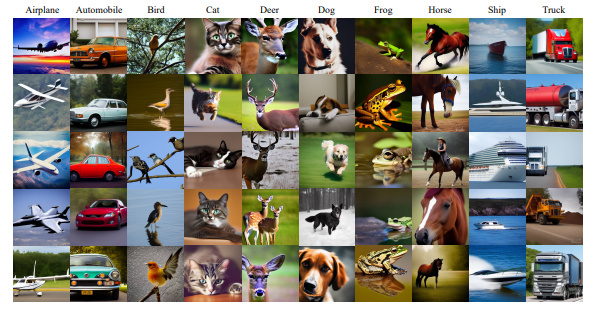
\includegraphics[width=0.76\textwidth]{images/q3_sdm_samples.png}
  \caption{Examples of synthetic images generated by SDM from the CIFAKE dataset \cite{bird_2023}}
  \label{fig:sdm_samples}
\end{figure}

Some visual defects are present in the samples of Figure \ref{fig:sdm_samples}, such as a one-winged bird and mis-shapen fighter jet tail. However, for the majority of examples, an untrained human cannot distinguish between real and synthetic. This would be especially true if the synthetic image were presented as real, either by unintentional misattribution or a deliberate intent to mislead. Compared to the above, which are generated by SDM, models like Imagen produce even more photorealistic images, as determined by human raters, also within a matter of seconds \cite{saharia_2022}.

There is, therefore, a justified increasing concern surrounding the possible malicious applications of AI image generation. For example, synthetic images have been used in the creation of fake journalist profiles and social media accounts, which can then be used to perpetuate fraud schemes and disinformation campaigns \cite{khoo_2021}.

\subsection{Literature Review}

Unsurprisingly, there is a reasonable research interest in the use of computer vision and image classification techniques to discriminate real and AI-generated synthetic images. Sha et al. \cite{sha_2023} suggest that frequency analysis can separate real images from images generated by diffusion models, and for the latter, may even provide information on which diffusion model generated the image. This is corroborated by Corvi et al. \cite{corvi_2022}, who extend the investigation to GAN-generated images (GAN: generative adversarial network; an alternative technique to LDMs for image synthesis). They find that individual GAN and diffusion models can be uniquely distinguished by the Fourier transform of their generated images \cite{corvi_2022}.

Furthermore, Amerini et al. \cite{amerini_2019} demonstrate an 81.61\% accuracy in discriminating original and deepfake videos by training CNNs (VGG16 and ResNet-50) on optical flow. Guera and Delp \cite{guera_2018} also use a CNN (InceptionV3) for frame-by-frame feature extraction from video, then use an LSTM (long short-term memory; a type of neural network specifically for sequential data) to process the sequence of features. They achieve 97\% accuracy in detecting deepfakes \cite{guera_2018}. Saikia et al. \cite{saikia_2022} combine the two approaches by training a hybrid CNN-LSTM model on optical flow. They test various CNNs pre-trained on the ImageNet dataset, including VGG16, InceptionV3 and ResNet-50, finding that ResNet-50 as a base model achieves the best accuracy of 89.67\% \cite{saikia_2022}. Wang et al. \cite{wang_2022} present a different approach, applying the transformer architecture to the deepfake problem. Transformers have gained significant traction in recent years as powerfully general model backbones for any machine learning task. Wang et al. \cite{wang_2022} report a state-of-the-art 97.93\% accuracy on the FaceForensics++ dataset.

Returning to images rather than videos, Guarnera et al. \cite{guarnera_2023} test ResNet-18 and ResNet-34, both pre-trained on ImageNet, on a dataset of real images and synthetic images generated by both GANs and LDMs. They achieve an accuracy of 95.24\% with ResNet-18, and 97.63\% with ResNet-34 \cite{guarnera_2023}. Guarnera et al. extend this investigation to a three-tier hierarchical classification task \cite{guarnera_2023}. At the first level, a ResNet is trained to classify images as real or synthetic \cite{guarnera_2023}. At the second level, another ResNet is trained to classify the source of predicted-synthetic images as either a GAN or LDM \cite{guarnera_2023}. Finally, given a GAN or LDM prediction, a third ResNet is trained to classify the specific model of origin; for example, StyleGAN or or Dall-E 2 \cite{guarnera_2023}. Both ResNet-18 and ResNet-34 achieve above 95\% accuracy on all tasks \cite{guarnera_2023}, suggesting a high degree of separability not only between real and synthetic, but even between sources of synthetic images. This again corroborates the results of \cite{corvi_2022} and \cite{sha_2023}.

Finally, Bird and Lotfi \cite{bird_2023} introduce the CIFAKE dataset, which consists of 60,000 synthetic images generated by SDM and 60,000 real images collected from CIFAR-10. CIFAR-10 is a dataset of small images, containing 6000 examples of each of 10 classes \cite{krizhevsky_2009}. These classes are: airplane, automobile, bird, cat, deer, dog, frog, horse, ship and truck \cite{krizhevsky_2009}. An equal number of images of identical classes compliments this to create the CIFAKE dataset \cite{bird_2023}. The images are generated by prompting SDM with the class name and one of several prompt modifiers, which are described in \cite{bird_2023}. Bird and Lotfi \cite{bird_2023} propose a simple CNN to discriminate real and fake images, and achieve a best result of 92.93\% on the CIFAKE dataset. This was achieved by a model with 2 layers of 128 filters \cite{bird_2023}.

\newpage
\section{Methodology}
\subsection{Classifier Architectures}

The review of the existing literature suggests an approach to the CIFAKE dataset. ResNet models pre-trained on the ImageNet dataset commonly achieve respectable results in discriminating real and fake images and videos. In particular, ResNet-18 and ResNet-34 are suitable candidates given their fast training times and the competitive results reported by \cite{guarnera_2023}. However, the highest reported accuracy is by the transformer model of \cite{wang_2022}. Therefore, this report will also investigate the performance of ViT-B/16 (Vision Transformer Base with 16 $\times$ 16 input patch size, from \cite{dosovitskiy_2021}) pre-trained on the ImageNet dataset. At the time of writing, Vision Transformers continue to rank among the state-of-the-art on the ImageNet classification dataset \cite{paperswithcode_2023}; ViT-B/16 represents the smallest of the pre-trained ViT models available from PyTorch \cite{torchcontributors_visiontransformer}.

Finally, a PCA and logistic regression benchmark is proposed for comparison to the results of ResNet-18, ResNet-34 and ViT-B/16. Despite the apparent proficiency of the current AI image generation techniques, the reviewed literature frequently reports high accuracy in discriminating the outputs of such techniques and real images. Even the simple CNN of \cite{bird_2023} achieves over 92\% accuracy on CIFAKE. Therefore, it is of interest to determine if the use of deep neural networks is justified, or if much simpler techniques remain able to discriminate the outputs of current AI image generation techniques.

\subsection{CIFAKE Dataset}

The CIFAKE dataset used in this investigation is freely available on the Kaggle platform \cite{bird_2023b}. The training data of 100,000 images is randomly split into a 20\% validation set and remaining training set. Each model uses an identical validation split by seeding the splitting process. Images are resized from 32x32 to 224x224 using bilinear interpolation before batching. All of this is facilitated by the Python fastai library, overlaying the PyTorch deep learning library.

\subsection{Logistic Regression Benchmark}

The PCA and logistic regression benchmark is constructed by flattening each training and testing image into a vector. PCA is used to determine the principal components of the training data, and the top 2, 5, 10, 20, 50 and 100 components are used in separate trials to transform both the training and testing images. A logistic regression model is fitted to the transformed training images and associated labels, then used to predict labels for the transformed testing images. Both the PCA and logistic regression implementations are from the skikit-learn library.

\subsection{Model Training}

All models are downloaded with pre-trained weights; the ResNets from PyTorch, and the ViT from PyTorch Image Models (timm). The models are loaded and fine-tuned using the fastai API. The default batch size of 64 is used, and a validation metric of error rate is reported. The default cross-entropy loss function is also retained. The models are fine-tuned using fastai until the validation loss does not decrease for two consecutive epochs. The state of the model after the epoch with the lowest validation loss is retained as the final model.

\subsection{Model Testing}

The trained models are tested by running inference on the dedicated test set of 20,000 images. Again, this is accomplished using the fastai API. The accuracy of each model is reported in the following section. All code is provided for reference in Appendix \ref{app:real_vs_fake_ipynb}.

\section{Results}

\subsection{Logistic Regression Benchmark}

Table \ref{tab:logistic_regression_benchmark} summarises the results of fitting a logistic regression model to varying numbers of the principal components of the training data.

\begin{table}[ht]
  \centering \small \restretch{1.5}
  \caption{Logistic regression accuracy using top N training data principal components}
  \begin{tabular}{lcrrrrrr}
    \toprule
    \textbf{N} (\#PC)  & & 2     & 5     & 10    & 20    & 50    & 100 \\
    \midrule
    \textbf{Acc.} (\%) & & 59.46 & 60.30 & 62.13 & 62.73 & 64.99 & 66.40 \\
    \bottomrule
  \end{tabular}
  \label{tab:logistic_regression_benchmark}
\end{table}

An asymptotic trend is evident, where each additional principal component contributes a lesser improvement in accuracy. This is the expected outcome, as the principal components are selected in order of decreasing explained variance. Using the top 100 principal components, an accuracy of 66.40\% is achieved using logistic regression. This result is only 16.40\% better than guessing at random, which provides good indication that the 92\% accuracy on CIFAKE of \cite{bird_2023} is a non-trivial result. The expectation is therefore set for the models to come.

\subsection{Model Results}

The following two figures present training loss as dashed lines, and validation loss as solid lines.

\begin{figure}[!ht]
  \centering
  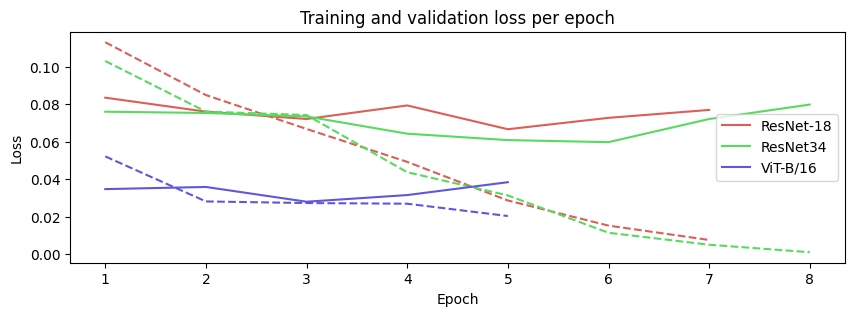
\includegraphics[width=0.95\textwidth]{images/q3_loss_per_epoch.png}
  \caption{Training and validation loss per epoch for each model}
  \label{fig:loss_per_epoch}
\end{figure}

\begin{figure}[!ht]
  \centering
  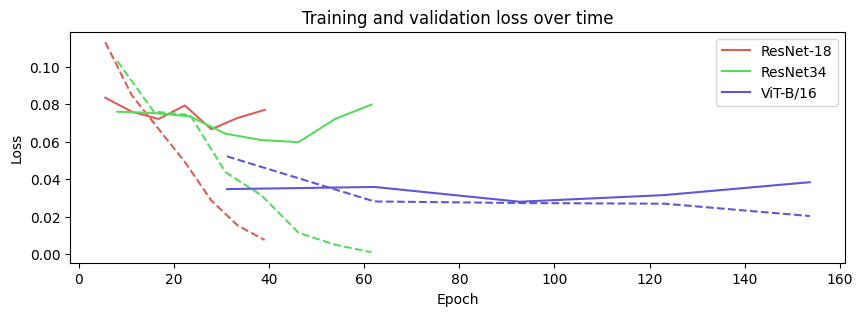
\includegraphics[width=0.95\textwidth]{images/q3_loss_per_time.png}
  \caption{Training and validation loss per epoch scaled by individual epoch durations}
  \label{fig:loss_per_time}
\end{figure}

\newpage

Table \ref{tab:model_results} summarises the training statistics of each model and the final test accuracy.

\begin{table}[ht]
  \centering \small \restretch{1.2}
  \caption{Model training and testing summaries}
  \begin{tabular}{lccccc}
    \toprule
    Model & Params & Avg. Epoch (mm:ss) & Tot. Time (hh:mm) & Final Val. Loss & Test Acc. (\%) \\
    \midrule
    ResNet-18 & 11.7M & 05:35 & 00:44 & 0.066654 & 97.89 \\
    ResNet-34 & 21.7M & 07:41 & 01:08 & 0.059770 & 98.19 \\
    ViT-B/16  & 86.6M & 30:44 & 02:58 & \textbf{0.028000} & \textbf{98.97} \\
    \bottomrule
  \end{tabular}
  \label{tab:model_results}
\end{table}

The model sizes in Table \ref{tab:model_results} are from the PyTorch documentation, rounded to the nearest 0.1M. Note that the average epoch is provided in minutes and seconds, whereas the total training time is provided in hours and minutes. The total time includes overhead, and is greater than the sum of the epochs.

\section{Discussion}

This report has presented an evaluation of two residual networks and one vision transformer on the CIFAKE dataset. The specific networks evaluated are: ResNet-18, ResNet-34 and ViT-B/16. A PCA and logistic regression baseline is also provided, and demonstrates that the problem of discriminating real and AI-generated images is not a trivial one. This is perhaps unsurprising, given the task is becoming near-impossible for even a human to complete with any reasonable accuracy. Despite this, the investigation finds that all networks successfully discriminate the real and generated images with an accuracy in every case exceeding 97\%.

ResNet-18 and ResNet-34 were selected based on their successful application to similar problems in the literature, by \cite{amerini_2019}, \cite{guarnera_2023} and \cite{saikia_2022}. In a particularly similar vein to this investigation, \cite{guarnera_2023} applies ResNet-18 and ResNet-34 to discriminate real and AI-generated images. They achieve not only a high accuracy in their primary task, but also in discriminating generated images by their source; either GAN or LDM, and even by the specific GAN or LDM model \cite{guarnera_2023}. This investigation corroborates the effectiveness of the ResNet architecture, with ResNet-18 and ResNet-34 achieving 97.89\% and 98.19\% on the CIFAKE dataset, respectively. This is achieved with less than an hour of training for the former, and only slightly more than an hour for the latter. Even so, Figure \ref{fig:loss_per_epoch} suggests that the validation loss of both ResNets decreases only marginally after the first epoch. To investigate this further, both were trained for only one epoch then tested. The results are 97.35\% and 97.76\% for ResNet-18 and ResNet-35, respectively, which supports the observation. This implies that a more efficient early-stopping condition should monitor the gradient of the loss per epoch, rather than the absolute value.

The findings are similar for the ViT. ViT-B/16 achieves 98.97\% accuracy on the CIFAKE dataset, possibly representing the new state-of-the-art and far exceeding the 92.93\% accuracy reported by \cite{bird_2023}. Training ViT-B/16 took an average of half an hour per epoch, and three hours in total. However, once again, Figure \ref{fig:loss_per_epoch} suggests that the validation loss decreases almost negligibly after the first epoch, even more so than for the ResNets. Due to the relatively long training duration of the ViT, this is not confirmed in a similar manner to the ResNets. However, there is strong implication that the same changes to the early-stopping condition for the ResNets apply to the ViT also.

The observed training behaviour of all three models, where improvement after the first epoch is marginal, is presumed to be an indication of effective transfer learning. Inspecting the fastai source code, the fine-tuning method occurs in two stages. For the first epoch (denoted epoch 0 in the output), all layers except the last are frozen. Frozen layers do not have their weights updated, meaning training occurs much faster. Following this, the entire model is unfrozen and the desired number of epochs is trained. It is possible that for all three models, their feature extraction layers are sufficiently general that only the classifier at the head of the model requires fine-tuning to achieve a high accuracy on the CIFAKE data. This is investigated on ResNet-18 by manually freezing the model up to the final layer and training a single epoch. The resulting model achieves 92.42\% accuracy on the test set, thus supporting the hypothesis. This suggests that a fast solution to the classification problem is to freeze the models up to the last layer and train for a single epoch. If more accuracy is required, a larger model may be chosen and/or the model can be unfrozen and trained for one more epoch.

Finally, comparing the three models, ViT-B/16 is superior where maximum accuracy is desired, but ResNet-18 represents the best ratio between accuracy and training time. The ViT is by far the largest model, larger even by parameter count than the largest ResNet, ResNet-152. Furthermore, ViTs and other transformer-based architectures currently demonstrate state-of-the-art performance in most applications, including image classification. Therefore, the performance of ViT-B/16 is well within expectation. However, practically, the accuracy of ViT-B/16 over ResNet-18 may be of minimal significance to most applications. For example, from the statistics of Table \ref{tab:model_results}, given the CIFAKE test set of 20,000 images, the ViT correctly classifies only 216 examples more than the ResNet-18, yet requires six times the training duration. Hence, it is presently difficult to justify the use of the ViT. However, as the proficiency of AI image generation continues to improve, the more performant architectures like ViTs could forseeably become a necessity to discriminate real and generated images in the near future.

\section{Conclusion}

In summary, this report presents an evaluation of three pre-trained models on the CIFAKE dataset, chosen for their success on similar tasks in the literature. The investigation finds that all three achieve $>$97\% accuracy, with performance improving with model size. The investigation also finds that both ResNets, and presumably also the ViT, achieve $>$97\% after fine-tuning for only one epoch. This indicates high transfer learning effectiveness, and suggests a time-saving strategy where some accuracy can be forgone. The investigation concludes with a direct comparison of the practical utility of the models. Given the large difference in training time but minimal improvement in accuracy, it is presently difficult to justify practical application of the larger models over ResNet-18. However, as AI image generation continues to improve, the more performant models may become necessary sooner rather than later.
